\begin{figure*}[h]
    \vspace{0.25cm}
    \centering
    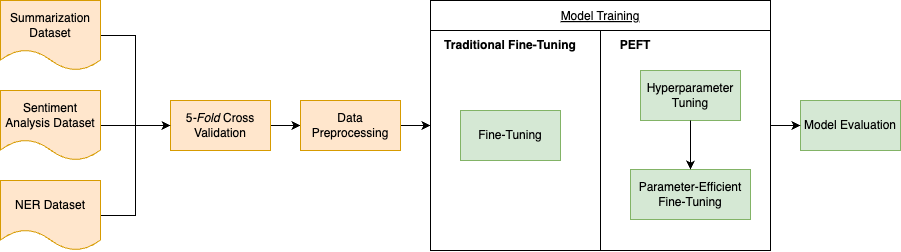
\includegraphics[width=0.8\textwidth]{resources/paper_solution.png}
    \caption{Methodology Workflow}
    \label{methodology}
\end{figure*}

\section{Methodology}

This study applies various Parameter-Efficient Fine-Tuning (PEFT) methods—Adapter, Low-Rank Adaptation (LoRA), Prefix-Tuning, and UniPELT—to IndoLEM tasks: Named Entity Recognition (NER), Sentiment Analysis, and Summarization. Figure \ref{methodology} outlines the overall workflow, starting with dataset preparation, followed by 5-fold cross-validation and data preprocessing. The models are trained using both traditional fine-tuning and PEFT methods, and their performance is evaluated using task-specific metrics such as F1 and ROUGE scores. 

The following subsections provide details on dataset preparation, training procedure, experiment design, and reproducibility.

\subsection{Dataset Preparation}

\begin{table}[htbp]
    \vspace{0.25cm}
    \centering
    \caption{Dataset Details}
    \label{table:dataset-indolem}
    \resizebox{0.5\textwidth}{!}{
    \begin{tabular}{lrrrcc}
        \toprule
        \textbf{Data} & \textbf{\#train} & \textbf{\#dev} & \textbf{\#test} & \textbf{5-fold} & \textbf{Evaluation} \\
        \midrule
        NER UGM & 1.530 & 170 & 425 & \checkmark & micro-averaged F1 \\
        NER UI & 1.687 & 187 & 469 & \checkmark & micro-averaged F1 \\
        \textit{Sentiment Analysis} & 3.638 & 399 & 1.011 & \checkmark & F1 \\
        IndoSum & 14.262 & 750 & 3.762 & \checkmark & ROUGE \\
        \bottomrule
    \end{tabular}
    }
\end{table}

The datasets used in this study were obtained from the IndoLEM benchmark, which provides annotated data for NER, Sentiment Analysis, and Summarization tasks. Each dataset underwent careful pre-processing to ensure compatibility with the selected PEFT methods.

\begin{itemize}
    \item \textbf{NER Task}: The NER datasets contain labeled entities such as persons, organizations, and locations. The goal is to identify and classify these entities within the text.
    \item \textbf{Sentiment Analysis Task}: The Sentiment Analysis dataset is categorized into positive, negative, and neutral classes, assessing the sentiment expressed in the text.
    \item \textbf{Summarization Task}: The Summarization dataset consists of pairs of original texts and their corresponding summaries, requiring models to generate concise summaries while retaining key information.
\end{itemize}

Pre-processing steps involved tokenization, sequence padding, and converting labels into formats required by the model architectures. Details of the datasets used are provided in Table \ref{table:dataset-indolem}.

\subsection{Training Procedure}

The training of each PEFT method was conducted using the Hugging Face Transformers library and the Adapters library. Two pre-trained models, IndoBERT and IndoT5, were chosen as the base models due to their strong performance in Indonesian language tasks and their suitability for different NLP tasks.

IndoBERT is a variant of the BERT model, pre-trained specifically on large Indonesian text corpora. BERT (Bidirectional Encoder Representations from Transformers) is designed to capture deep bidirectional representations by conditioning on both left and right context in all layers. This characteristic makes IndoBERT highly effective for classification tasks, where understanding the full context of a sentence or sequence is crucial. In this study, IndoBERT was used as the base model for two key classification tasks: Named Entity Recognition (NER) and Sentiment Analysis. For NER, IndoBERT was fine-tuned using various PEFT methods to classify and identify entities such as persons, organizations, and locations in the text. For Sentiment Analysis, IndoBERT was fine-tuned to classify text into positive, negative, or neutral sentiment categories. IndoBERT’s ability to handle both sentence-level and token-level classification tasks makes it an ideal choice for both NER and Sentiment Analysis, capturing both the global context of a sentence and the fine-grained token-level distinctions needed for entity recognition.

On the other hand, IndoT5 (a variant of the Text-to-Text Transfer Transformer or T5) is better suited for generation tasks like Summarization. Unlike BERT, which is designed for classification tasks, T5 is designed to treat all NLP problems as text-to-text tasks, where both the input and output are text sequences. This characteristic makes IndoT5 particularly effective for generating new text, such as concise summaries of longer documents. In this study, IndoT5 was used as the base model for the Summarization task, where it was fine-tuned to generate accurate and concise summaries from input text, while retaining the most important information.

Each PEFT method was applied in distinct ways:
\begin{itemize}
    \item \textbf{Adapter}: Small bottleneck layers were added within each Transformer layer of IndoBERT and IndoT5, with only these adapters being updated during fine-tuning.
    \item \textbf{LoRA}: Weight matrices in the models were decomposed into low-rank matrices, enabling efficient adaptation by modifying a small fraction of the parameters.
    \item \textbf{Prefix-Tuning}: Trainable prefix tokens were prepended to the input sequences, and only these tokens were optimized during training.
    \item \textbf{UniPELT}: Combined different PEFT methods dynamically during training for a flexible approach.
\end{itemize}

Training hyperparameters such as learning rate, batch size, and epochs were selected based on previous research. Details are available in the experimental setup script. The training process used NVIDIA Tesla V100 for NER and Sentiment Analysis tasks, while NVIDIA A40 was used for Summarization.


\subsection{Experiment Design}

\begin{table}[htbp]
    \centering
    \caption{PEFT Configuration}
    \label{table:peft-configuration}
    \begin{tabular}{l|l|c}
        \toprule
        \textbf{Method} & \textbf{Argument} & \textbf{Value} \\
        \midrule
        LoRA & \texttt{rank} & [8, 16] \\
        Prefix Tuning & \texttt{prefix\_length} & [5, 50] \\
        Adapter & \texttt{reduction\_factor} & [64, 16] \\
        UniPELT & \multicolumn{1}{c|}{-}  & - \\
        \bottomrule
    \end{tabular}
\end{table}

The experiment design focused on two primary objectives:
\begin{itemize}
    \item \textbf{Parameter Efficiency}: Measure the number of trainable parameters for each PEFT method, comparing them to the traditional fine-tuning approach. The reduction in parameters is expected to lead to more efficient model training and deployment.
    \item \textbf{Training Time}: Evaluate how each PEFT method impacts training time across different tasks, aiming to achieve faster training without compromising performance.
\end{itemize}

Table \ref{table:peft-configuration} shows the key configurations for each PEFT method. For instance, LoRA experiments varied the rank between 8 and 16, impacting the model's adaptability and parameter count. Prefix-Tuning experiments tested prefix lengths of 5 and 50, exploring trade-offs between context length and training speed. Adapter experiments utilized reduction factors of 64 and 16, balancing parameter reduction with adaptability. UniPELT used its default dynamic configuration.

The experiments were designed to explore how these configurations affected computational efficiency and task performance. Each experiment included baseline traditional fine-tuning for comparison.

The performance of the models was evaluated using the same metrics as in the original IndoLEM paper. These metrics include:

\begin{itemize}
    \item \textbf{NER}: The evaluation used entity-level metrics, including accuracy, precision, recall, and F1 score. These metrics assess how well the model identifies and classifies entities (e.g., persons, organizations, locations) within the text.
    \item \textbf{Sentiment Analysis}: Evaluated using accuracy, precision, recall, and F1 score, which measure the model's ability to classify text into positive, negative, or neutral sentiment categories.
    \item \textbf{Summarization}: Measured using ROUGE-1, ROUGE-2, and ROUGE-L to compare generated summaries with reference texts, evaluating how well the model captures important content from the original text.
\end{itemize}

\subsection{Reproducibility and Code Availability}

Ensuring the reproducibility of the results was a key consideration in this study. All code developed for data processing, model training, and evaluation is publicly available in a GitHub repository (\url{https://github.com/apwic/indolem-peft}), complete with clear documentation. This transparency allows other researchers to replicate the experiments and build upon this work, further advancing the field of NLP for the Indonesian language.

